% Created 2023-01-11 Qua 10:15
% Intended LaTeX compiler: pdflatex
\documentclass[article,12pt,openany,oneside,a4paper,chapter=TITLE,hyphen,english,brazil,chapter=TITLE,sumario=tradicional]{abntex2}
              \usepackage{nopageno}
\usepackage{pdfpages}
\usepackage{times}
\usepackage[utf8]{inputenc}
\usepackage[T1]{fontenc}
\usepackage{color}
\usepackage{microtype}
\usepackage{titlesec}
\usepackage[brazilian, hyperpageref]{backref}
\usepackage{hyperref}
\usepackage[alf,abnt-emphasize=bf,abnt-doi=link]{abntex2cite}
\usepackage{indentfirst}
\usepackage{listings}
\usepackage{graphicx}
\usepackage{lipsum}
\usepackage{amssymb}
\usepackage{amsmath}
\lstset{basicstyle=\ttfamily\small,breaklines=true}
\titleformat{\section}{\normalfont\normalsize\bfseries\uppercase}{}{0pt}{}
\titleformat{\subsection}{\normalfont\normalsize\bfseries}{}{0pt}{\space}
\titleformat{\subsubsection}{\normalfont\normalsize\bfseries}{}{0pt}{\space}
\titleformat{\paragraph}{\normalfont\normalsize\itshape}{}{0pt}{\theparagraph\space}
\setlength{\parindent}{1.5cm}
\setlrmarginsandblock{3cm}{2cm}{*}
\setulmarginsandblock{2.5cm}{2.5cm}{*}
\checkandfixthelayout
\renewcommand{\backrefpagesname}{Citado na(s) página(s):~}
\renewcommand{\backref}{}
\renewcommand*{\backrefalt}[4]{}
\makeindex
\titulo{Partitura para Oficina de Música de Curitiba 2023}
\author{Davi Raubach}
\local{Pelotas}
\author{Davi Raubach}
\date{}
\title{omcwb}
\hypersetup{
 pdfauthor={Davi Raubach},
 pdftitle={omcwb},
 pdfkeywords={},
 pdfsubject={},
 pdfcreator={Emacs 29.0.50 (Org mode 9.5.4)}, 
 pdflang={Bt-Br}}
\begin{document}

\OnehalfSpacing

\pretextual

\imprimircapa
\newpage

\begin{dedicatoria}
\vspace*{\fill}
Esta é uma dedicatória.

\vspace*{\fill}
\end{dedicatoria}
\newpage

\begin{epigrafe}
\vspace*{\fill}
Nunca nos curamos de ter sonhado ao pé de uma água dormente\ldots{}
Gaston Bachelard
\vspace*{\fill}
\end{epigrafe}
\newpage



\textual


\section*{Prefácio}
\label{sec:org978633b}
Nesta composição, a leitura de um texto verbal ocupa uma posição de geração de material musical e de organizador relativo da temporalidade. Em boa parte da peça, o passar do tempo é articulado pela leitura do texto.

O poema abaixo cumpre essa função na peça foi escrito para essa ocasião.

\begin{center}


Palavra atirada contra a água\\
Salta, salta, voa\\
Pousa sobre as nuvens\\
Mergulha cada vez mais fundo\\
Cada vez mais alto\\
Seduz a língua e escoa\\
Escoa, salta, voa\\
Cada vez mais sonhada
\end{center}


\section*{Notas de Performance}
\label{sec:org38a70ba}

\textbf{Duração} c. 4 min

\subsection*{Notação rítmica}
\label{sec:org1083797}
\subsubsection*{Tempo estrito}
\label{sec:org737850d}
Notado tradicionalmente
\subsubsection*{Tempo de fala}
\label{sec:org8f27409}
Gestos instrumentais estão associados às sílabas do texto. O/A intérprete deve executar a música levando em conta sua associação com o texto. Uma leitura mental é que determina quando tocar. Pontos e vírgulas podem ser interpretados como pausas, fraseseado e dinâmicas podem derivar também do texto.

Cabeça de nota como de semínima representa a leitura de uma sílaba para cada nota (notas mais curtas). Cabeça de nota como de mínimas representam notas que se estendem por várias sílabas (notas mais longas):

\begin{center}
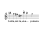
\includegraphics[width=7cm]{exemplo_tempo_fala.pdf}
\end{center}


Em geral, o ritmo instrumental deve se submeter ao ritmo da leitura. Entretanto, também deve-se levar em consideração que alguns gestos precisam de tempo hábil para a exeucução e nestes casos não há problema em suspender o tempo da leitura.


\includepdf[pages=-,pagecommand={}]{omcwb_score.pdf}
\end{document}